\chapter{Specifikacija programske potpore}

\section{Funkcionalni zahtjevi}


\noindent \textbf{Dionici:}

\begin{packed_enum}
	
	\item Pacijent
	\item Zaposlenik (medicinsko osoblje)				
	\item Administrator
	\item Razvojni tim:
	\begin{packed_item}
		\item Dora Kašik (voditelj)
		\item Josip Begić
		\item Erik Greblo
		\item Anton Vivoda
		\item Roko Krstičević
		\item Katarina Mikulić
		\item Marko Miletić
	\end{packed_item}
	
\end{packed_enum}

\noindent \textbf{Aktori i njihovi funkcionalni zahtjevi:}


\begin{packed_enum}
	\item  \underbar{Pacijent (inicijator) može:}
	
	\begin{packed_enum}
		
		\item Predati zahtjev za terapijom i dodjelom termina iste
		\begin{packed_enum}
			
			\item  Ako dolazi na ponovljenu terapiju, u zahtjevu prilaže referencu na prethodno obavljenu terapiju
			
		\end{packed_enum}
		\item Izvršiti registraciju u sustav
		
		
	\end{packed_enum}
	
	\item  \underbar{Administrator (inicijator) može:}
	
	\begin{packed_enum}
		
		\item Upravljati  podacima o pacijentima i djelatnicima
		\item Upravljati podacima o dostupnoj opremi i prostorijama klinike
		\item Vršiti postupke za zaštitu podataka
		\item Dodavati nove djelatnike
		
	\end{packed_enum}
	
	\item  \underbar{Superadministrator (inicijator) može:}
	
	\begin{packed_enum}
		
		\item Dodijeliti djelatniku administratorskih ovlasti
		\item Ukloniti administratorske ovlasti djelatnika
		\item Verificirati registraciju korisnika
		\item Upravljati  podacima o pacijentima i djelatnicima
		\item Upravljati podacima o dostupnoj opremi i prostorijama klinike
		\item Vršiti postupke za zaštitu podataka
		\item Dodavati nove djelatnike
		
	\end{packed_enum}
	
	\item  \underbar{Zaposlenik (inicijator) može:}
	
	\begin{packed_enum}
		
		\item Dodijeliti termin pacijentu
		\begin{packed_enum}
			
			\item Nakon dodjele termina šalje pacijentu potrebne podatke o terminu putem elektroničke pošte
			
		\end{packed_enum}
		\item Pristupiti pregledu aktivnih prijava pacijenata
		\item Pristupiti podatku o dostupnim djelatnicima
		\item Pristupiti podatku o trajanju pojedinog zahvata
		\item Pristupiti podacima o dostupnoj opremi i prostorijama klinike
		\item Registrirati dolazak pacijenta na terapiju i rezultate nakon obavljene terapije
		\item Prihvatiti ili odbiti zahtjev pacijenta za terminom terapije
		
		
	\end{packed_enum}
	
	\item  \underbar{Baza podataka (sudionik) može:}
	
	\begin{packed_enum}
		
		\item Pohranjuje podatke o korisnicima i njihovim ovlastima
		\item Pohranjuje podatke o terapijama
		\item Pohranjuje podatke o čestim pitanjima
		\item Pohranjuje podatke o prostorijama i opremi
		
	\end{packed_enum}
	
\end{packed_enum}

\eject 



\subsection{Obrasci uporabe}


\subsubsection{Opis obrazaca uporabe}


\noindent \underbar{\textbf{UC1 - Registracija pacijenta}}
\begin{packed_item}
	
	\item \textbf{Glavni sudionik: }Pacijent
	\item  \textbf{Cilj:} Registracija novog pacijenta u sustavu
	\item  \textbf{Sudionici:} Baza podataka/Sustav
	\item  \textbf{Preduvjet:} Bolesnik nema prethodno registriran račun
	\item  \textbf{Opis osnovnog tijeka:}
	
	\item[] \begin{packed_enum}
		
		\item Pacijent unosi osobne podatke, adresu elektroničke pošte i lozinku.
		\item Sustav provjerava ispravnost podataka.
		\item Sustav pohranjuje podatke i stvara korisnički račun.
		
	\end{packed_enum}
	
	\item  \textbf{Opis mogućih odstupanja:} Ako podaci nisu ispravni, sustav obavještava korisnika o potrebnim ispravkama.
	
	
\end{packed_item}

\noindent \underbar{\textbf{UC2 - Prijava pacijenta}}
\begin{packed_item}
	
	\item \textbf{Glavni sudionik: }Pacijent
	\item  \textbf{Cilj:} Pristup stranici rehabilitacije nakon prijave
	\item  \textbf{Sudionici:} Baza podataka
	\item  \textbf{Preduvjet:} Pacijent je registriran i prijavljen u sustav
	\item  \textbf{Opis osnovnog tijeka:}
	
	\item[] \begin{packed_enum}
		
		\item Pacijent šalje zahtjev za prijavom na sustav s korisničkim imenom i lozinkom.
		\item Sustav provjerava ispravnost podataka.
		\item Ako su podaci ispravni, pacijent je prijavljen u sustav.
		
	\end{packed_enum}
	
	\item  \textbf{Opis mogućih odstupanja:} Ako podaci nisu ispravni, sustav obavještava korisnika o potrebnim ispravkama. Ako pacijent nije registriran, sustav obavještava korisnika da nema važeći račun. 
	
	
\end{packed_item}

\noindent \underbar{\textbf{UC3 - Zahtjev za resetiranje lozinke}}
\begin{packed_item}
	
	\item \textbf{Glavni sudionik: }Pacijent
	\item  \textbf{Cilj:} Prijava u sustav kako bi pristupio stranici rehabilitacije
	\item  \textbf{Sudionici:} Baza podataka/Sustav
	\item  \textbf{Preduvjet:} Korisnik ima registriran račun u sustavu
	\item  \textbf{Opis osnovnog tijeka:}
	
	\item[] \begin{packed_enum}
		
		\item Pacijent šalje zahtjev za poveznicu za resetiranje lozinke
		\item Sustav šalje poveznicu za resetiranje lozinke na korisnikovu adresu elektroničke pošte.
		
	\end{packed_enum}
	
	\item  \textbf{Opis mogućih odstupanja:} Ako se ne može pronaći korisnik s unesenom adresom e-pošte, sustav obavještava korisnika o neuspjelom zahtjevu. 
	
	
\end{packed_item}

\noindent \underbar{\textbf{UC4 - Spremanje nove lozinke}}
\begin{packed_item}
	
	\item \textbf{Glavni sudionik: }Pacijent
	\item  \textbf{Cilj:} Spremiti novu lozinku nakon poveznice za resetiranje lozinke
	\item  \textbf{Sudionici:} Baza podataka/Sustav
	\item  \textbf{Preduvjet:} Korisnik je primio poveznicu za resetiranje lozinke i želi postaviti novu lozinku
	\item  \textbf{Opis osnovnog tijeka:}
	
	\item[] \begin{packed_enum}
		
		\item Pacijent šalje novu lozinku putem poveznice za resetiranje lozinke.
		\item Sustav sprema novu lozinku za korisnički račun.
		
	\end{packed_enum}
	
	\item  \textbf{Opis mogućih odstupanja:} Ako poveznica za resetiranje lozinke nije ispravna ili je istekla, sustav obavještava korisnika o neuspjelom ažuriranju lozinke. 
	
	
\end{packed_item}

\noindent \underbar{\textbf{UC5 - Dodavanje zaposlenika u bazu}}
\begin{packed_item}
	
	\item \textbf{Glavni sudionik: }Superadministrator
	\item  \textbf{Cilj:} Registrirati novog zaposlenika u sustavu
	\item  \textbf{Sudionici:} Baza podataka/Sustav
	\item  \textbf{Preduvjet:} Korisnik ima superadministratorske ovlasti i prijavljen je u sustav
	\item  \textbf{Opis osnovnog tijeka:}
	
	\item[] \begin{packed_enum}
		
		\item Superadministrator šalje zahtjev za registraciju zaposleniika s podacima o zaposleniku.
		\item Sustav provjerava ispravnost podataka.
		\item Sustav registrira zaposlenika u sustavu.
		
	\end{packed_enum}
	
	\item  \textbf{Opis mogućih odstupanja:} Ako podaci nisu ispravni, sustav obavještava superadministratoar o potrebnim ispravkama.
	
	
\end{packed_item}

\noindent \underbar{\textbf{UC6 - Brisanje zaposlenika}}
\begin{packed_item}
	
	\item \textbf{Glavni sudionik: }Superadministrator
	\item  \textbf{Cilj:} Deaktivirati račun određenog zaposlenika u sustav
	\item  \textbf{Sudionici:} Baza podataka/Sustav
	\item  \textbf{Preduvjet:} Korisnik ima superadministratorske ovlasti i prijavljen je u sustav
	\item  \textbf{Opis osnovnog tijeka:}
	
	\item[] \begin{packed_enum}
		
		\item Superadministrator šalje zahtjev za brisanje zaposlenika s određenim identifikatorom.
		\item Sustav označava zaposlenika kao neaktivnog u bazi podataka.
		
	\end{packed_enum}
	
	
\end{packed_item}

\noindent \underbar{\textbf{UC7 - Dodavanje učestalih pitanja (FAQ)}}
\begin{packed_item}
	
	\item \textbf{Glavni sudionik: }Administrator
	\item  \textbf{Cilj:} Dodati novi FAQ u sustav
	\item  \textbf{Sudionici:} Baza podataka/Sustav
	\item  \textbf{Preduvjet:} Korisnik ima administratorske ovlasti i prijavljen je u sustav
	\item  \textbf{Opis osnovnog tijeka:}
	
	\item[] \begin{packed_enum}
		
		\item Administrator šalje zahtjev za dodavanje novog FAQ-a s podacima o FAQ-u.
		\item Sustav provjerava ispravnost podataka.
		\item Sustav dodaje novi FAQ u sustav.
		
	\end{packed_enum}
	
	\item  \textbf{Opis mogućih odstupanja:} Ako podaci nisu ispravni, sustav obavještava administratora o potrebnim ispravkama.
	
	
\end{packed_item}

\noindent \underbar{\textbf{UC8 - Prikaz svih učestalih pitanja (FAQ-a)}}
\begin{packed_item}
	
	\item \textbf{Glavni sudionik: }Bilo koji korisnik
	\item  \textbf{Cilj:} Prikazati popis svih FAQ-ova u sustavu
	\item  \textbf{Sudionici:} Baza podataka/Sustav
	\item  \textbf{Opis osnovnog tijeka:}
	
	\item[] \begin{packed_enum}
		
		\item Korisnik šalje zahtjev za dohvaćanje svih FAQ-ova.
		\item Sustav dohvaća popis FAQ-ova iz baze podataka.
		\item Sustav vraća odgovor s popisom FAQ-ova.
		
	\end{packed_enum}
	
	
\end{packed_item}

\noindent \underbar{\textbf{UC9 - Brisanje učestalih pitanja (FAQ)}}
\begin{packed_item}
	
	\item \textbf{Glavni sudionik: }Administrator
	\item  \textbf{Cilj:} Brisati određeni FAQ iz sustava
	\item  \textbf{Sudionici:} Baza podataka/Sustav
	\item  \textbf{Preduvjet:} Korisnik ima administratorske ovlasti i prijavljen je u sustav
	\item  \textbf{Opis osnovnog tijeka:}
	
	\item[] \begin{packed_enum}
		
		\item Administrator šalje zahtjev za brisanje FAQ-a s određenim identifikatorom.
		\item Sustav označava FAQ kao neaktivan u bazi podataka.
		
	\end{packed_enum}
	
	
\end{packed_item}

\noindent \underbar{\textbf{UC10 - Kreiranje sobe}}
\begin{packed_item}
	
	\item \textbf{Glavni sudionik: }Superadministrator
	\item  \textbf{Cilj:} Kreirati novu sobu u sustavu
	\item  \textbf{Sudionici:} Baza podataka/Sustav
	\item  \textbf{Preduvjet:} Korisnik ima superadministratorske ovlasti i prijavljen je u sustav
	\item  \textbf{Opis osnovnog tijeka:}
	
	\item[] \begin{packed_enum}
		
		\item Superadministrator šalje zahtjev za kreiranje nove sobe s potrebnim podacima.
		\item Sustav provjerava ispravnost podataka.
		
	\end{packed_enum}
	
	\item  \textbf{Opis mogućih odstupanja:} Ako podaci nisu ispravni, sustav obavještava uperadministratora o potrebnim ispravkama.
	
	
\end{packed_item}

\noindent \underbar{\textbf{UC11 - Pregled svih soba}}
\begin{packed_item}
	
	\item \textbf{Glavni sudionik: }Zaposlenik
	\item  \textbf{Cilj:} Prikazati sve sobe u sustavu
	\item  \textbf{Sudionici:} Baza podataka/Sustav
	\item  \textbf{Preduvjet:} Korisnik ima administratorske ovlasti i prijavljen je u sustav
	\item  \textbf{Opis osnovnog tijeka:}
	
	\item[] \begin{packed_enum}
		
		\item Zaposlenik šalje zahtjev za dohvaćanje svih soba.
		\item Sustav dohvaća sve sobe iz baze podataka.
		\item Sustav vraća odgovor s popisom soba.
		
	\end{packed_enum}
	
	
\end{packed_item}

\noindent \underbar{\textbf{UC12 - Pregled sobe po identifikacijskom broju}}
\begin{packed_item}
	
	\item \textbf{Glavni sudionik: }Zaposlenik
	\item  \textbf{Cilj:} Pregledati pojedinu sobu u sustavu
	\item  \textbf{Sudionici:} Baza podataka/Sustav
	\item  \textbf{Preduvjet:} Korisnik ima administratorske ovlasti i prijavljen je u sustav
	\item  \textbf{Opis osnovnog tijeka:}
	
	\item[] \begin{packed_enum}
		
		\item Zaposlenik šalje zahtjev za dohvat sobe  s određenim identifikatorom.
		\item Sustav provjerava postoji li soba s navedenim identifikacijskim brojem.
		\item Ako postoji, sustav prikazuje podatke o sobi.
		
	\end{packed_enum}
	
	\item  \textbf{Opis mogućih odstupanja:} Ako soba s navedenim identifikacijskim brojem ne postoji, sustav obavještava zaposlenika.
	
	
\end{packed_item}

\noindent \underbar{\textbf{UC13 - Brisanje sobe}}
\begin{packed_item}
	
	\item \textbf{Glavni sudionik: }Superadministrator
	\item  \textbf{Cilj:} Obrisati sobu iz sustava
	\item  \textbf{Sudionici:} Baza podataka/Sustav
	\item  \textbf{Preduvjet:} Korisnik ima superadministratorske ovlasti i prijavljen je u sustav
	\item  \textbf{Opis osnovnog tijeka:}
	
	\item[] \begin{packed_enum}
		
		\item Superadministrator šalje zahtjev za brisanje sobe s određenim identifikacijskim brojem.
		\item Sustav provjerava postoji li soba s navedenim identifikacijskim brojem.
		\item Ako postoji, sustav briše sobu.
		
	\end{packed_enum}
	
	\item  \textbf{Opis mogućih odstupanja:} Ako podaci nisu ispravni, sustav obavještava administratora o potrebnim ispravkama.
	
	
\end{packed_item}

\noindent \underbar{\textbf{UC14 - Kreiranje opreme}}
\begin{packed_item}
	
	\item \textbf{Glavni sudionik: }Superadministrator
	\item  \textbf{Cilj:} Kreirati novu opremu u sustavu
	\item  \textbf{Sudionici:} Baza podataka/Sustav
	\item  \textbf{Preduvjet:} Korisnik ima superadministratorske ovlasti i prijavljen je u sustav
	\item  \textbf{Opis osnovnog tijeka:}
	
	\item[] \begin{packed_enum}
		
		\item Superadministrator šalje zahtjev za kreiranje nove opreme s potrebnim podacima.
		\item Sustav provjerava ispravnost podataka.
		\item Sustav kreira novu opremu u sustav.
		
	\end{packed_enum}
	
	\item  \textbf{Opis mogućih odstupanja:} Ako podaci nisu ispravni, sustav obavještava superadministratora o potrebnim ispravkama.
	
	
\end{packed_item}

\noindent \underbar{\textbf{UC15 - Pregled svih oprema}}
\begin{packed_item}
	
	\item \textbf{Glavni sudionik: }Zaposlenik
	\item  \textbf{Cilj:} Prikazati sve sobe u sustavu
	\item  \textbf{Sudionici:} Baza podataka/Sustav
	\item  \textbf{Preduvjet:} Korisnik ima administratorske ovlasti i prijavljen je u sustav
	\item  \textbf{Opis osnovnog tijeka:}
	
	\item[] \begin{packed_enum}
		
		\item Zaposlenik šalje zahtjev za dohvaćanje svih oprema.
		\item Sustav dohvaća svu opremu iz baze podataka.
		\item Sustav vraća odgovor s popisom opreme.
		
	\end{packed_enum}
	
\end{packed_item}

\noindent \underbar{\textbf{UC16 - Pregled opreme po identifikacijskom broju}}
\begin{packed_item}
	
	\item \textbf{Glavni sudionik: }Zaposlenik
	\item  \textbf{Cilj:} Pregledati pojedinu opremu u sustavu
	\item  \textbf{Sudionici:} Baza podataka/Sustav
	\item  \textbf{Preduvjet:} Korisnik ima administratorske ovlasti i prijavljen je u sustav
	\item  \textbf{Opis osnovnog tijeka:}
	
	\item[] \begin{packed_enum}
		
		\item Zaposlenik šalje zahtjev za dohvat opreme s određenim identifikatorom.
		\item Sustav provjerava postoji li oprema s navedenim identifikacijskim brojem.
		\item Ako postoji, sustav prikazuje podatke o opremi.
		
	\end{packed_enum}
	
	\item  \textbf{Opis mogućih odstupanja:} Ako oprema s navedenim identifikacijskim brojem ne postoji, sustav obavještava zaposlenika.
	
	
\end{packed_item}

\noindent \underbar{\textbf{UC17 - Brisanje opreme}}
\begin{packed_item}
	
	\item \textbf{Glavni sudionik: }Superadministrator
	\item  \textbf{Cilj:} Obrisati opremu iz sustava
	\item  \textbf{Sudionici:} Baza podataka/Sustav
	\item  \textbf{Preduvjet:} Korisnik ima superadministratorske ovlasti i prijavljen je u sustav
	\item  \textbf{Opis osnovnog tijeka:}
	
	\item[] \begin{packed_enum}
		
		\item Superadministrator šalje zahtjev za brisanje opreme s određenim identifikacijskim brojem.
		\item Sustav sustav provjerava postoji li oprema s navedenim identifikacijskim brojem.
		\item Ako postoji, sustav briše opremu.
		
	\end{packed_enum}
	
	
\end{packed_item}

\noindent \underbar{\textbf{UC18 - Prikaz svih pacijenata}}
\begin{packed_item}
	
	\item \textbf{Glavni sudionik: }Administrator
	\item  \textbf{Cilj:} Prikazati popis svih pacijenata u sustavu
	\item  \textbf{Sudionici:} Baza podataka/Sustav
	\item  \textbf{Preduvjet:} Korisnik ima administratorske ovlasti i prijavljen je u sustav
	\item  \textbf{Opis osnovnog tijeka:}
	
	\item[] \begin{packed_enum}
		
		\item Administrator šalje zahtjev za dohvaćanje svih pacijenata.
		\item Sustav dohvaća popis pacijenata iz baze podataka.
		\item Sustav vraća odgovor s popisom pacijenata.
		
	\end{packed_enum}
	
	
\end{packed_item}

\noindent \underbar{\textbf{UC19 - Deaktivacija pacijentovog računa}}
\begin{packed_item}
	
	\item \textbf{Glavni sudionik: }Pacijent, Zaposlenik, Admin
	\item  \textbf{Cilj:} Deaktivirati račun određenog pacijenta u sustavu
	\item  \textbf{Sudionici:} Baza podataka/Sustav
	\item  \textbf{Preduvjet:} Korisnik je prijavljen u sustav
	\item  \textbf{Opis osnovnog tijeka:}
	
	\item[] \begin{packed_enum}
		
		\item Korisnik šalje zahtjev za deaktivaciju pacijentovog računa s određenim identifikatorom.
		\item Sustav označava pacijenta kao neaktivnog u bazi podataka.
		
	\end{packed_enum}
	
	
\end{packed_item}

\noindent \underbar{\textbf{UC20 - Kreiranje terapije za pacijenta}}
\begin{packed_item}
	\item \textbf{Glavni sudionik:} Pacijent, Zaposlenik
	\item \textbf{Cilj:} Dodati novu terapiju za određenog pacijenta
	\item \textbf{Sudionici:} Baza podataka/Sustav
	\item \textbf{Preduvjet:} Korisnik i zaposlenik prijavljeni u sustav
	\item \textbf{Opis osnovnog tijeka:}
	
	\begin{packed_enum}
		\item Korisnik šalje zahtjev za dodavanje nove terapije s podacima o terapiji.
		\item Sustav provjerava ispravnost unesenih podataka.
		\item Zaposlenik unosi dodatne informacije o terapiji poput datuma, vremena i sobe.
		\item Sustav provjerava valjanost unesenih podataka, uključujući dostupnost sobe i preklapanje termina.
		\item Ako su podaci valjani, terapija se odobrava zaposleniku i potvrđuje pacijentu.
	\end{packed_enum}
	
	\item \textbf{Opis mogućih odstupanja:} Ako podaci nisu ispravni, sustav obavještava korisnika o potrebnim ispravkama.
	
\end{packed_item}

\noindent \underbar{\textbf{UC21 - Prikaz svih terapija za pacijenta}}
\begin{packed_item}
	
	\item \textbf{Glavni sudionik: }Pacijent
	\item  \textbf{Cilj:} Prikazati popis svih terapija za određenog pacijenta
	\item  \textbf{Sudionici:} Baza podataka/Sustav
	\item  \textbf{Preduvjet:} Korisnik je prijavljen u sustav
	\item  \textbf{Opis osnovnog tijeka:}
	
	\item[] \begin{packed_enum}
		
		\item Korisnik šalje zahtjev za dohvaćanje svih terapija za određenog pacijenta.
		\item Sustav dohvaća popis terapija iz baze podataka za određenog pacijenta.
		\item Sustav vraća odgovor s popisom terapija.
		
	\end{packed_enum}
	
	
\end{packed_item}

\noindent \underbar{\textbf{UC22 - Unos rezultata terapije}}
\begin{packed_item}
	
	\item \textbf{Glavni sudionik: }Zaposlenik
	\item  \textbf{Cilj:} Unijeti rezultate terapije u sustav
	\item  \textbf{Sudionici:} Baza podataka/Sustav
	\item  \textbf{Preduvjet:} Korisnik ima ovlasti zaposlenika i prijavljen je u sustav
	\item  \textbf{Opis osnovnog tijeka:}
	
	\item[] \begin{packed_enum}
		
		\item Zaposlenik odabire pacijenta iz dostupne liste.
		\item Sustav provjerava bazu podataka kako bi dohvatio relevantne podatke o pacijentu.
		\item U slučaju uspješnog pronalaska pacijenta, zaposlenik šalje zahtjev za unos rezultata terapije, pružajući relevantne podatke o rezultatima.
		\item Sustav provjerava ispravnost unesenih podataka.
		\item Ako su podaci ispravni, sustav zabilježava rezultate terapije u bazu podataka.
		\item Nakon uspješnog zapisivanja, sustav prikazuje na zaslonu potvrdu o uspješno unesenom zapisu, pružajući zaposleniku vizualnu potvrdu.
		\item Pacijent ima mogućnost pregleda svojih rezultata terapije unutar web-aplikacije.
		
	\end{packed_enum}
	
	\item  \textbf{Opis mogućih odstupanja:} Ako podaci nisu ispravni, sustav obavještava zaposlenika o potrebnim ispravkama.
	
	
\end{packed_item}

\noindent \underbar{\textbf{UC23 - Dodjela administratorskih ovlasti}}
\begin{packed_item}
	
	\item \textbf{Glavni sudionik: }Superadministrator
	\item  \textbf{Cilj:} Dodjela administratorskih ovlasti radi lakšeg upravljanja sustavom
	\item  \textbf{Sudionici:} Baza podataka/Sustav
	\item  \textbf{Preduvjet:} Korisnik ima ovlasti superadministratora i prijavljen je u sustav
	\item  \textbf{Opis osnovnog tijeka:}
	
	\item[] \begin{packed_enum}
		
		\item Superadministator šalje zahtjev za dodjelu administratorskih ovlasti određenom korisniku.
		\item Sustav provjerava ispravnost zahtjeva i potvrđuje administratorske ovlasti korisniku.
		\item Sustav ažurira informacije o ovlastima korisnika u bazi podataka.
		
	\end{packed_enum}
	
	\item  \textbf{Opis mogućih odstupanja:} Ako podaci nisu ispravni ili korisnik već ima administratorske ovlasti, sustav obavještava superadministratora o potrebnim ispravkama ili prekoračenju ovlasti.
	
	
\end{packed_item}

\noindent \underbar{\textbf{UC24 - Uklanjanje administratorskih ovlasti}}
\begin{packed_item}
	
	\item \textbf{Glavni sudionik: }Superadministrator
	\item  \textbf{Cilj:} Uklanjanje administratorskih ovlasti korisniku u sustavu
	\item  \textbf{Sudionici:} Baza podataka/Sustav
	\item  \textbf{Preduvjet:} Korisnik ima ovlasti superadministratora i prijavljen je u sustav
	\item  \textbf{Opis osnovnog tijeka:}
	
	\item[] \begin{packed_enum}
		
		\item Administrator šalje zahtjev za uklanjanje administratorskih ovlasti određenom korisniku.
		\item Sustav provjerava ispravnost zahtjeva i uklanja administratorske ovlasti korisniku.
		\item Sustav ažurira informacije o ovlastima korisnika u bazi podataka.
		
	\end{packed_enum}
	
	\item  \textbf{Opis mogućih odstupanja:} Ako podaci nisu ispravni ili korisnik nema administratorske ovlasti, sustav obavještava administratora o potrebnim ispravkama ili nedostatku ovlasti za uklanjanje.
	
	
\end{packed_item}

\noindent \underbar{\textbf{UC25 - Prikaz svih zaposlenika}}
\begin{packed_item}
	
	\item \textbf{Glavni sudionik: }Administrator
	\item  \textbf{Cilj:} Prikazati popis svih zaposlenika u sustavu
	\item  \textbf{Sudionici:} Baza podataka/Sustav
	\item  \textbf{Preduvjet:} Korisnik ima administratorske ovlasti i prijavljen je u sustav
	\item  \textbf{Opis osnovnog tijeka:}
	
	\item[] \begin{packed_enum}
		
		\item Administrator šalje zahtjev za dohvaćanje svih djelatnika.
		\item Sustav dohvaća popis zaposlenika iz baze podataka.
		\item Sustav vraća odgovor s popisom zaposlenika.
		
	\end{packed_enum}
	
	
\end{packed_item}

\subsubsection{Dijagrami obrazaca uporabe}

\begin{figure}[H]
	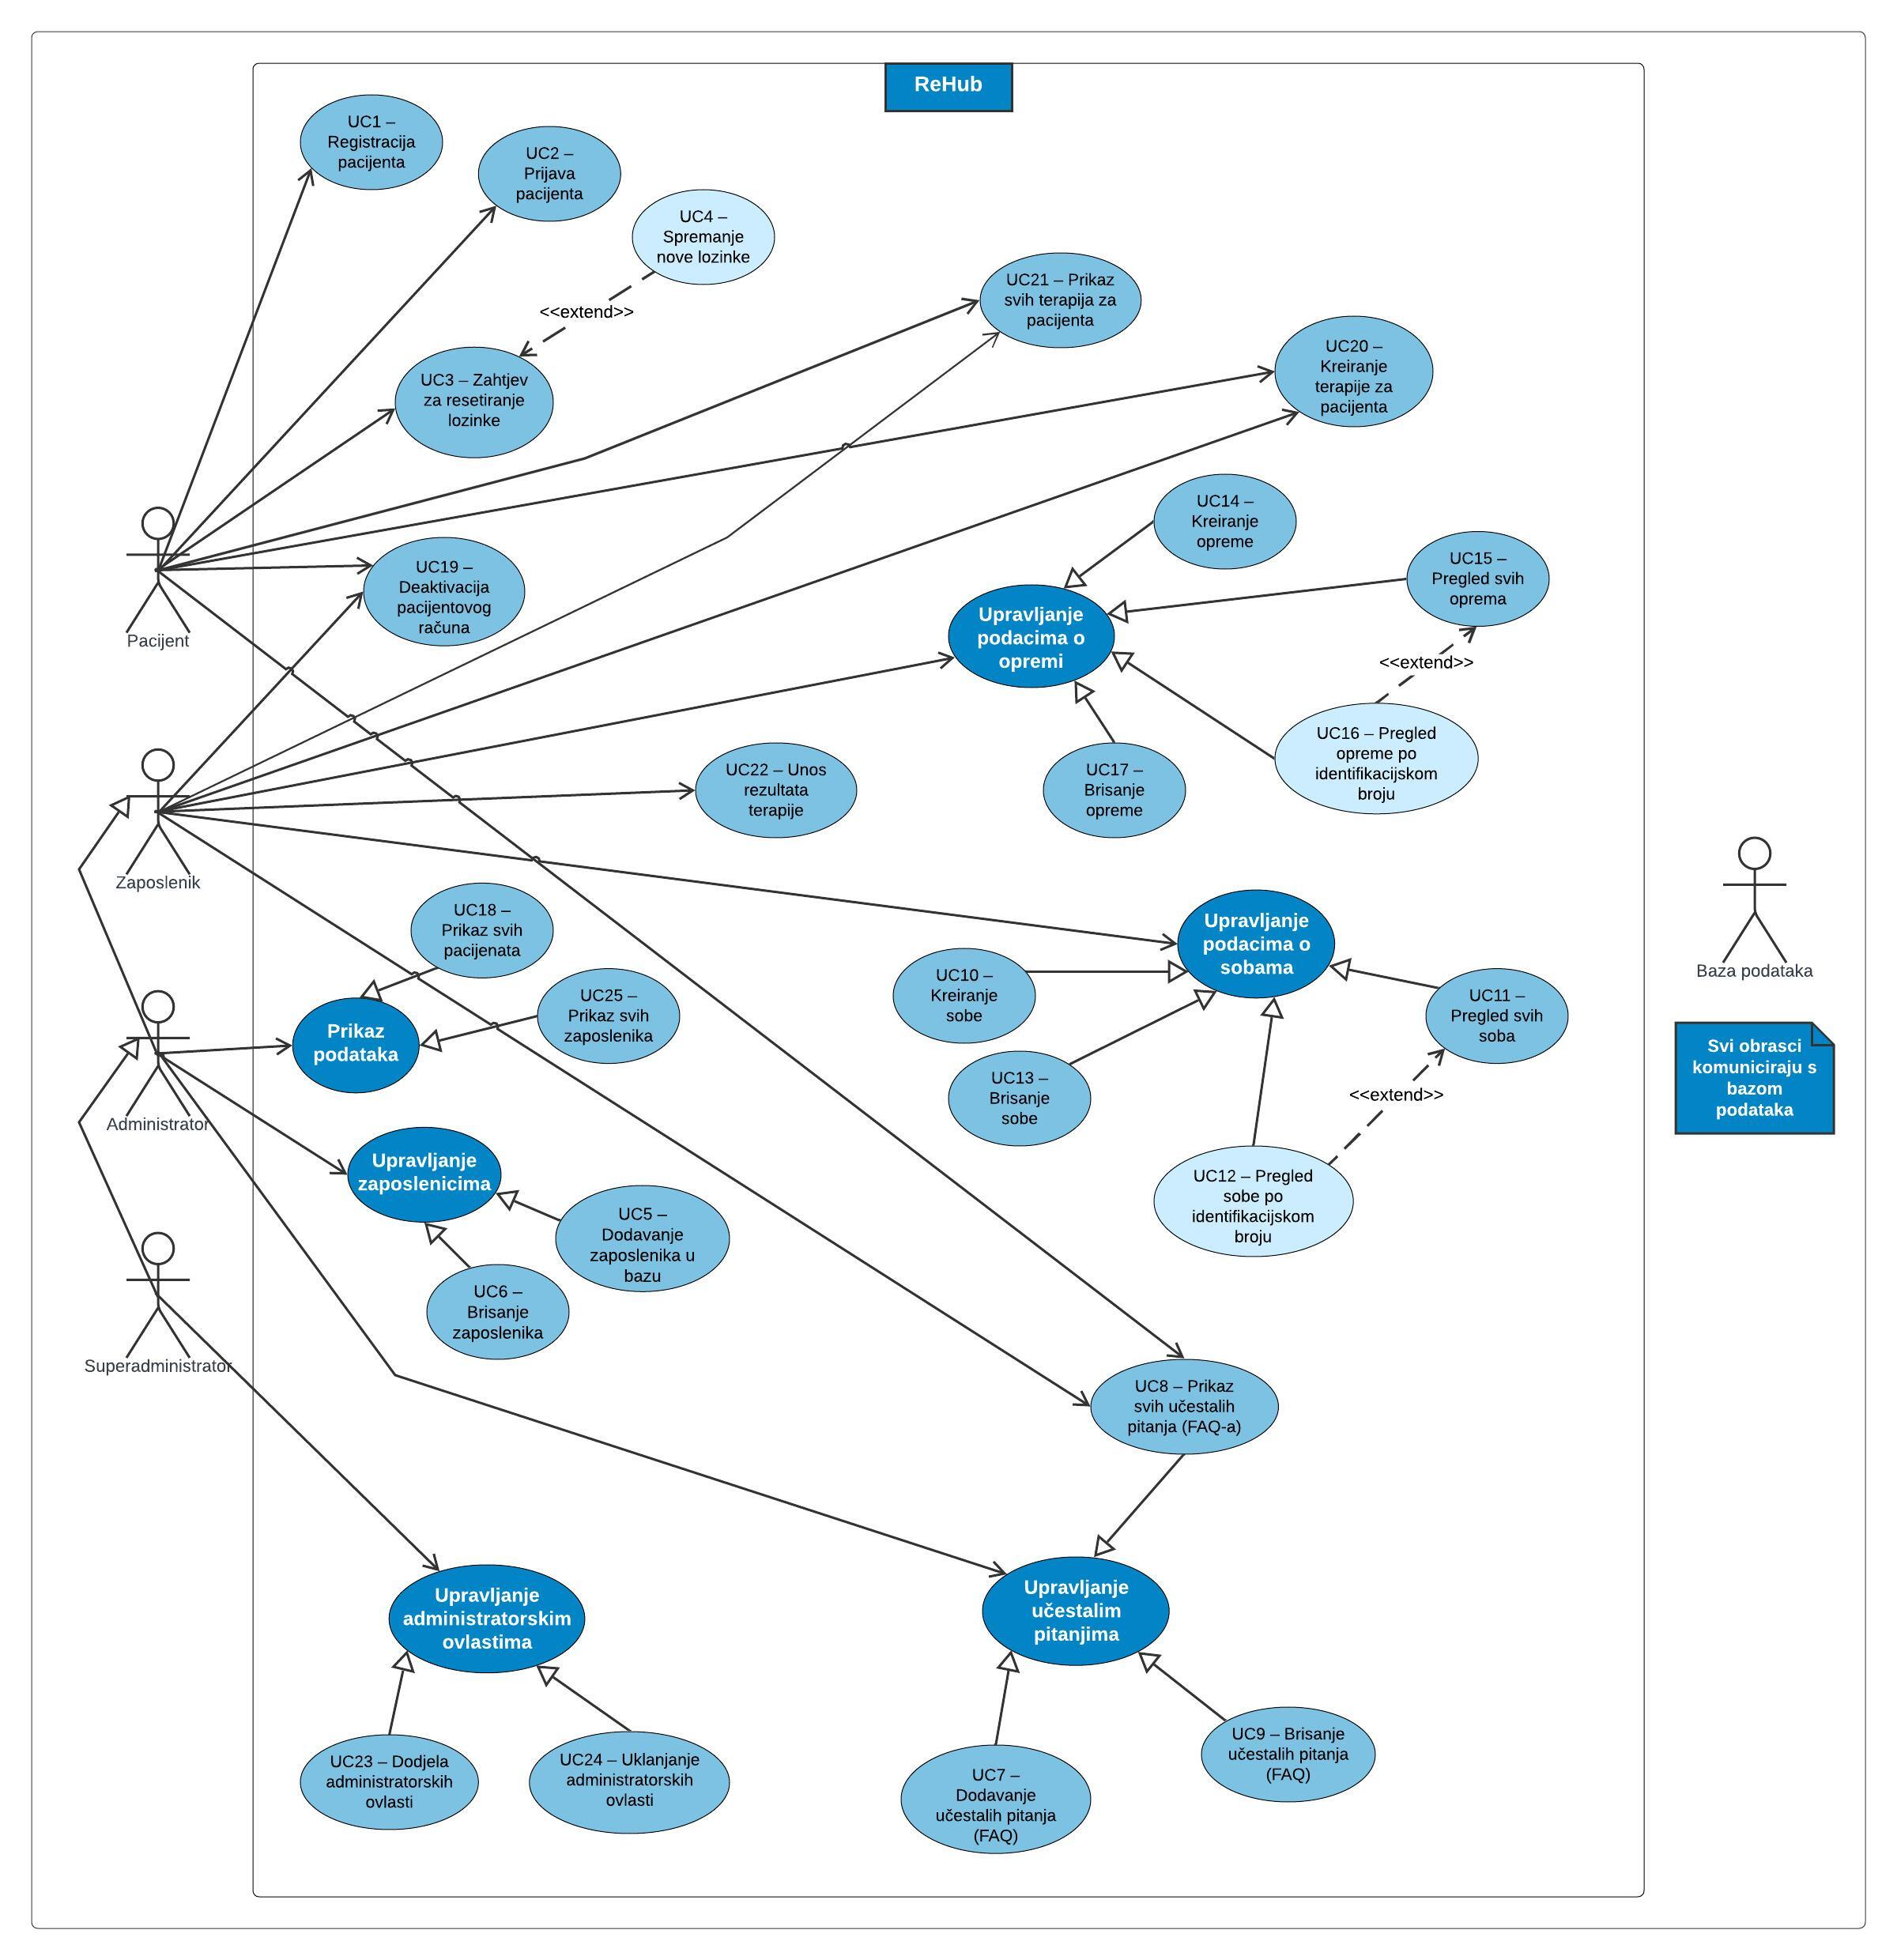
\includegraphics[scale=0.35]{dijagrami/ReHub Use case diagram.jpeg}
	\centering
	\caption{Dijagram obrazaca uporabe}
	\label{fig:UseCaseDiagram}
\end{figure}
\eject		

\subsection{Sekvencijski dijagrami}

U sljedećem dijelu prikazani su sekvencijski dijagrami i njihovi opisi.
\subsubsection{Obrazac uporabe UC5 – Dodavanje zaposlenika, UC6 - Brisanje zaposlenika i UC23 – Dodjela administratorskih ovlasti}


Kada korisnik odabere opciju "Dodavanje zaposlenika", web-aplikacija omogućuje korisniku unos svih relevantnih podataka o novom zaposleniku. Nakon završetka unosa, aplikacija automatski ažurira bazu podataka s novim informacijama.U slučaju odabira opcije "Brisanje zaposlenika", web-aplikacija pristupa bazi podataka kako bi prikazala popis trenutno zaposlenih osoba. Korisnik ima mogućnost odabira zaposlenika koje želi izbrisati, a nakon potvrde brisanja, aplikacija ažurira bazu podataka u skladu s korisnikovim zahtjevom. Kada korisnik odabere opciju "Dodjela administratorskih ovlasti", web-aplikacija pruža korisniku mogućnost odabira zaposlenika kojima želi dodijeliti administratorske ovlasti. Nakon što korisnik izabere zaposlenike, aplikacija ažurira bazu podataka s promijenjenim ovlastima za odabrane osobe. U situaciji kada baza podataka ne sadrži informacije o zaposlenicima u skladu s odabranim opcijama (primjerice, nema zaposlenika za brisanje ili dodjelu administratorskih ovlasti), web-aplikacija će prikazati odgovarajuću poruku, obavještavajući korisnika o nedostatku dostupnih podataka za izvršenje odabrane radnje.

\begin{figure}[H]
	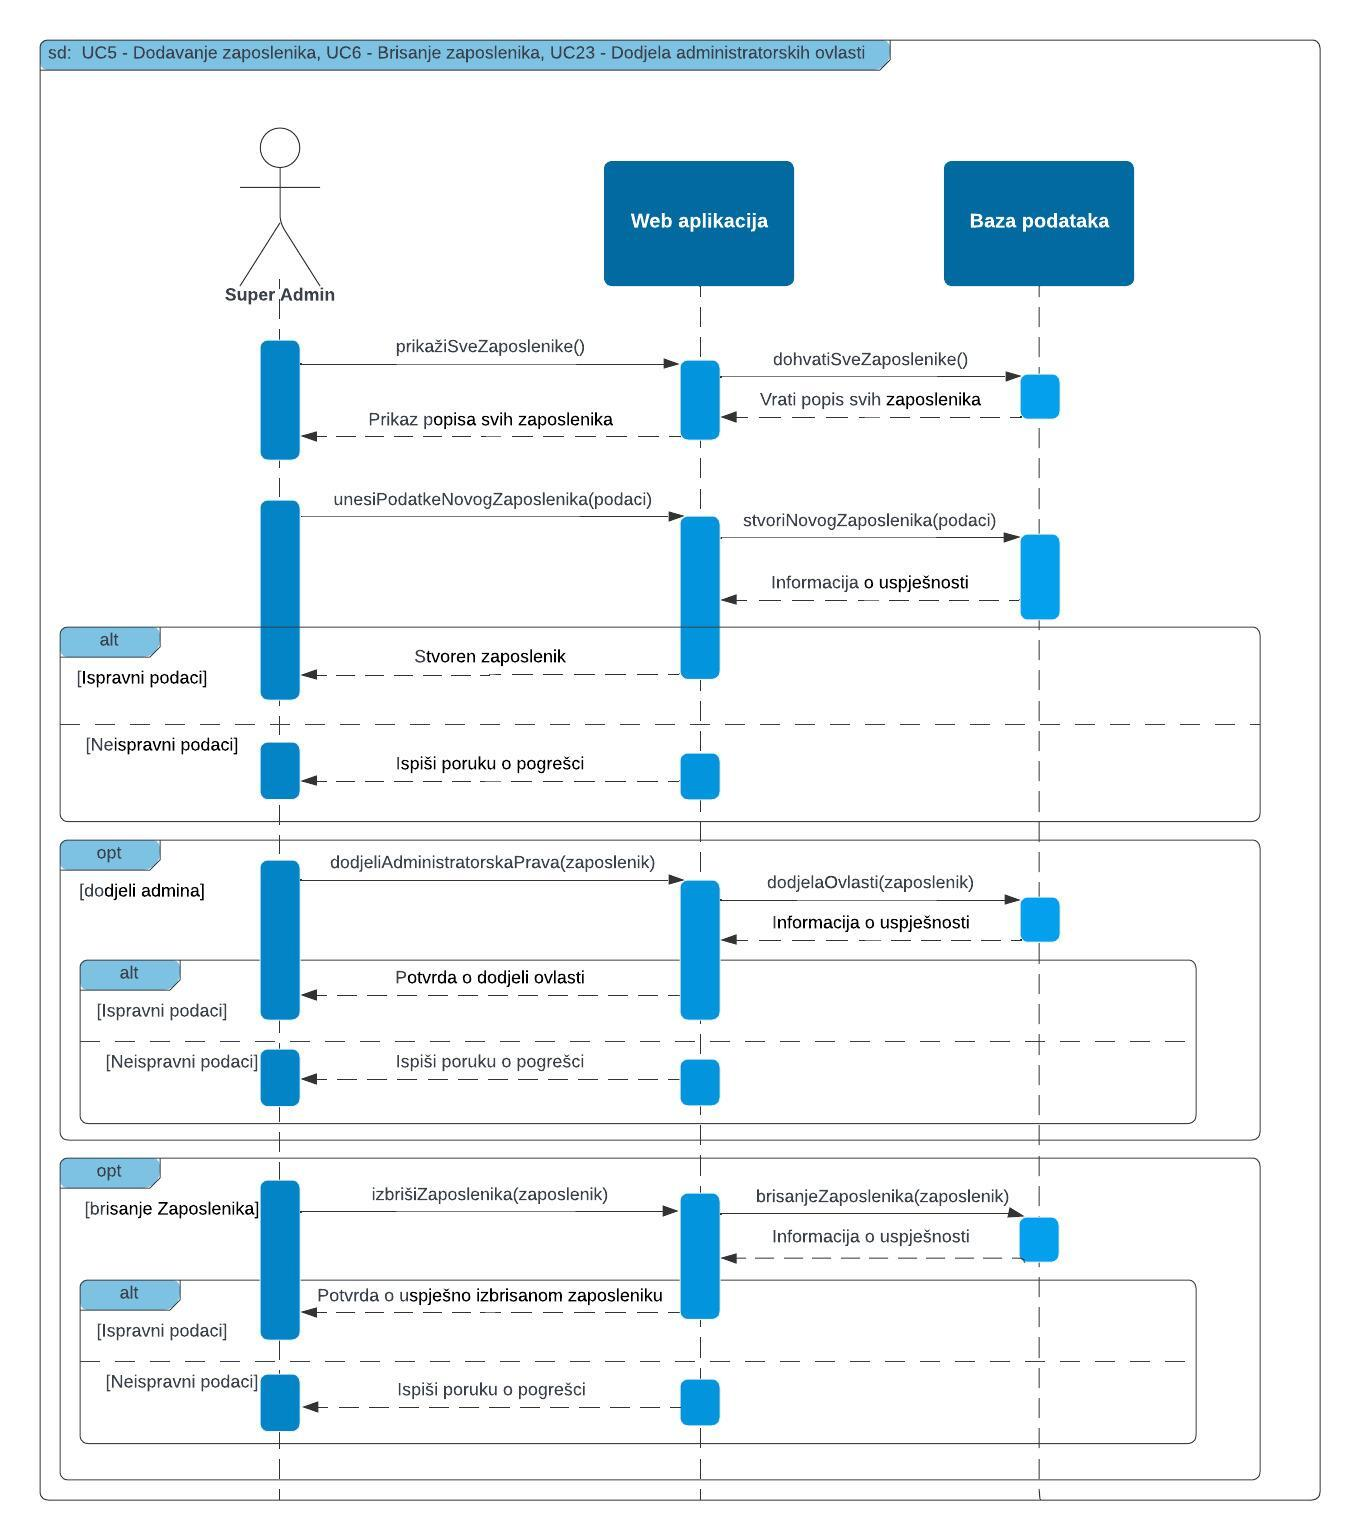
\includegraphics[scale=0.7]{dijagrami/Sequence diagram RH.jpeg}
	\centering
	\caption{Sekvencijski dijagram za UC5/6/23}
	\label{fig:SequenceDiagram1}
\end{figure}

\eject

\subsubsection{Obrazac uporabe UC22 - Unos rezultata terapije}

Kada zaposlenik pokreće proces unosa rezultata terapije, prvo odabire pacijenta iz dostupne liste. Nakon odabira pacijenta, web-aplikacija provjerava bazu podataka kako bi dohvatila relevantne podatke o tom pacijentu. Ako pacijent nije pronađen, sustav ispisuje poruku o pogrešci, obavještavajući zaposlenika o nedostatku informacija. U slučaju uspješnog pronalaska pacijenta, zaposlenik unosi rezultate terapije. Uneseni podaci o rezultatima terapije zatim se upisuju u bazu podataka. Nakon uspješnog zapisivanja, sustav prikazuje na zaslonu potvrdu o uspješno unesenom zapisu, pružajući zaposleniku vizualnu potvrdu. Dodatno, nakon unosa rezultata, pacijent ima mogućnost pregleda svojih rezultata terapije unutar web-aplikacije. To omogućuje pacijentu praćenje vlastitog napretka i informiranje o rezultatima terapije. 

\begin{figure}[H]
	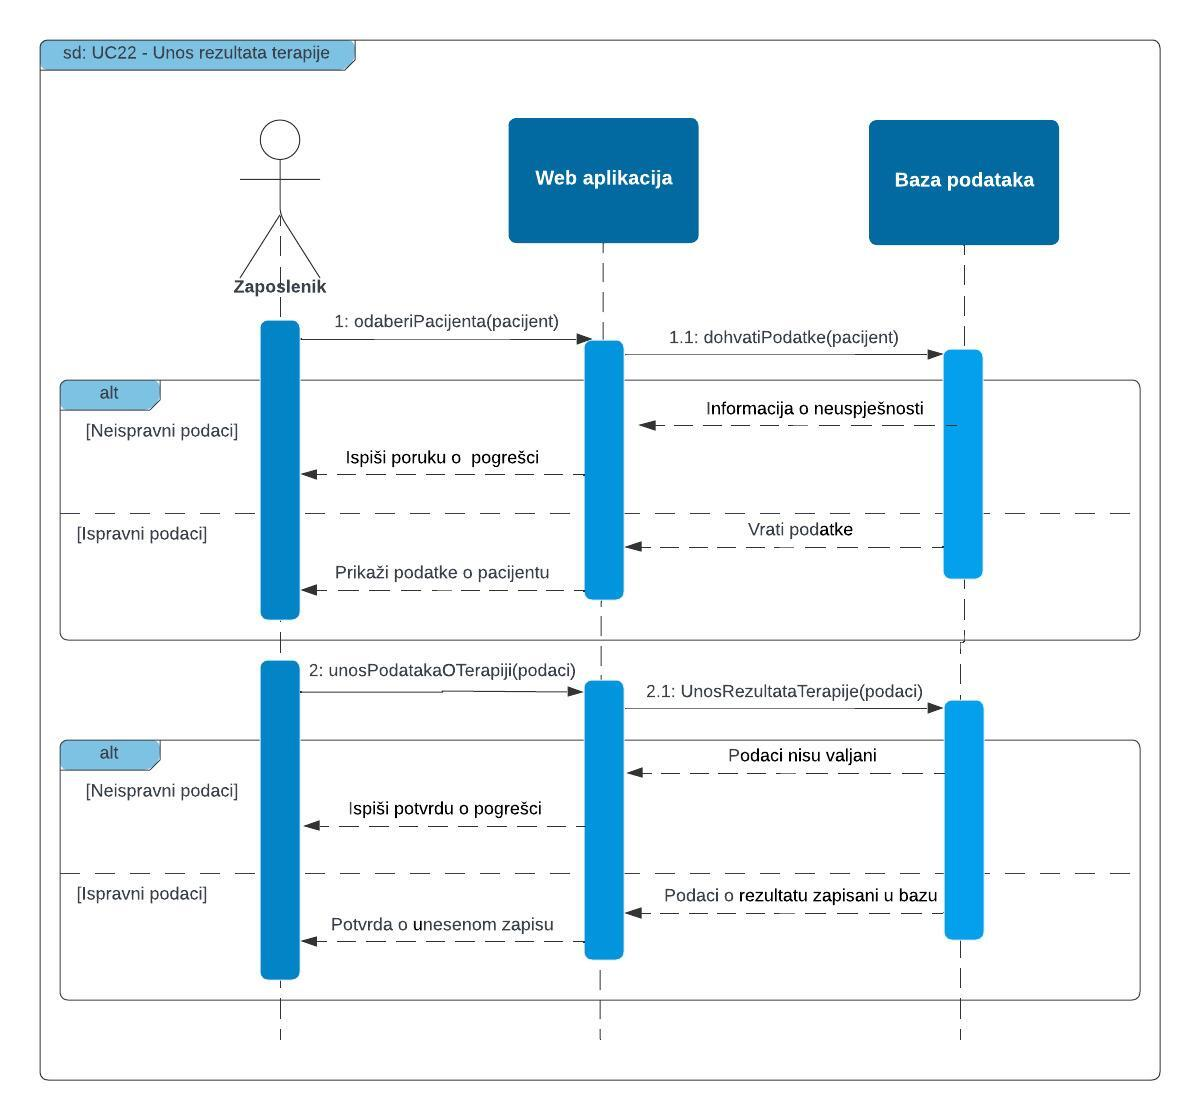
\includegraphics[scale=0.7]{dijagrami/Sequence diagram uc22.jpeg}
	\centering
	\caption{Sekvencijski dijagram za UC22}
	\label{fig:SequenceDiagram2}
\end{figure}

\eject

\subsubsection{Obrazac uporabe UC20 - Kreiranje terapije za pacijenta}


Kada pacijent zatraži obrazac za prijavu na rehabilitaciju, web-aplikacija generira i vraća prijavu. Pacijent unosi informacije o terapiji, a sustav provjerava ispravnost podataka u bazi. Ako su svi podaci ispravno uneseni, omogućuje se terapija, ali ostaje nepotvrđena. Liječniku se prikazuje zahtjev za terapijom, gdje unosi datum, vrijeme i sobu. Web-aplikacija provjerava valjanost unesenih podataka, uključujući dostupnost sobe i preklapanje termina. Ako su podaci valjani, terapija se potvrđuje, a pacijentu se odobrava. Pacijent prima potvrdu o odobrenju terapije, a dodatno može pregledavati svoje rezultate unutar aplikacije. Ovaj proces osigurava učinkovito upravljanje terapijama, pravovremenu potvrdu i omogućuje pacijentima praćenje vlastitog napretka.

\begin{figure}[H]
	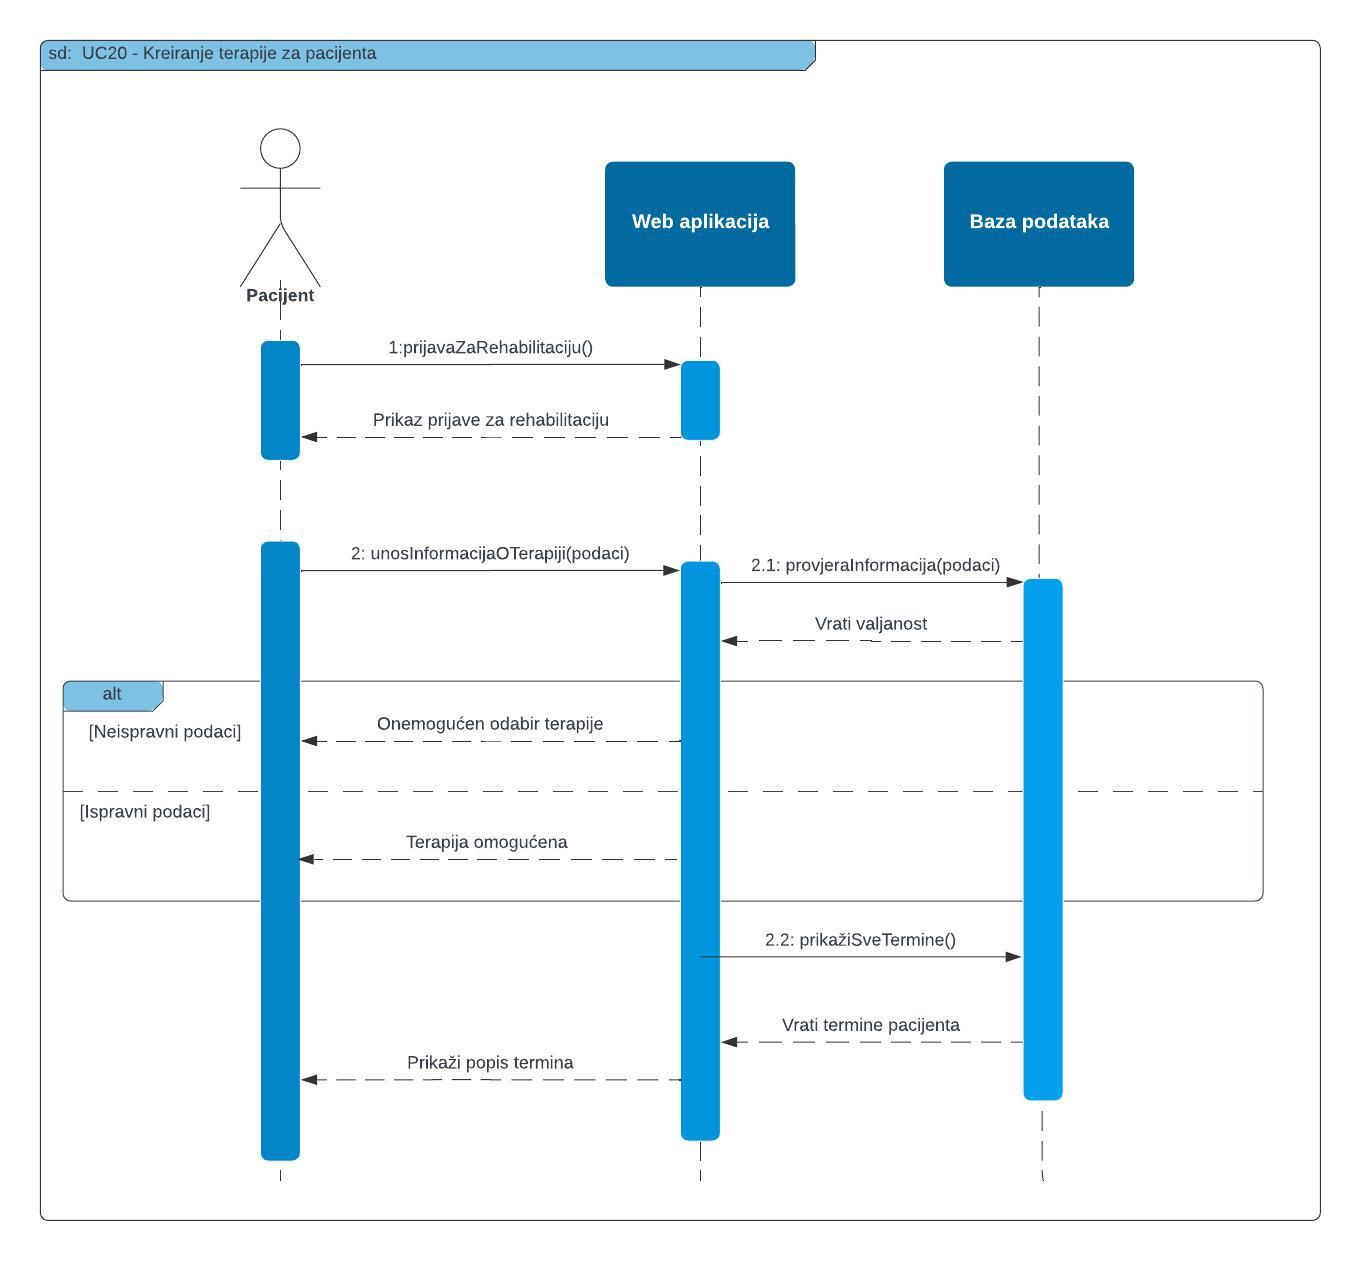
\includegraphics[scale=0.7]{dijagrami/Kreiranje terapije.jpeg}
	\centering
	\caption{Sekvencijski dijagram za UC20}
	\label{fig:SequenceDiagram3}
\end{figure}

\eject

\section{Ostali zahtjevi}

\begin{packed_enum}
	
	\large \item Sustav mora podržavati više različitih uloga korisnika \normalsize
	\begin{packed_item}
		\item Sustav treba omogućiti definiranje različitih razina pristupa i funkcionalnosti ovisno o ulozi korisnika (Administrator, Liječnik, Pacijent, itd.).
	\end{packed_item}
	\large \item Korisnički podaci moraju biti sigurno pohranjeni u sustavu	\normalsize
	\begin{packed_item}
		\item Sustav treba koristiti kriptiranje za pohranu i prijenos osjetljivih korisničkih podataka kako bi osigurao privatnost i sigurnost informacija.
	\end{packed_item}
	\large \item Brza i pouzdana veza s bazom podataka \normalsize
	\begin{packed_item}
		\item Sustav treba osigurati pouzdanu vezu s bazom podataka kako bi pristup podacima bio brz i otporan na vanjske pogreške.
	\end{packed_item}
	\large \item Odgovarajuće vrijeme izvršavanja za upite prema bazi podataka \normalsize
	\begin{packed_item}
		\item Izvršavanje upita koji pristupaju bazi podataka ne smije trajati dulje od definiranog vremena, kako bi se osigurala učinkovitost sustava.
	\end{packed_item}
	\large \item Podrška za hrvatsku abecedu u korisničkom sučelju i pri unosu teksta \normalsize
	\begin{packed_item}
		\item Korisničko sučelje i sustav trebaju podržavati hrvatsku abecedu pri unosu, prikazu i obradi tekstualnih podataka.
	\end{packed_item}
	\large \item Web aplikacija implementirana korištenjem objektno-orijentiranih jezika \normalsize
	\begin{packed_item}
		\item Sustav treba biti implementiran kao web aplikacija koristeći suvremene objektno-orijentirane jezike kako bi bio skalabilan i održiv.
	\end{packed_item}
	\large \item Intuitivan i lagan za korištenje \normalsize
	\begin{packed_item}
		\item Korisničko sučelje treba biti intuitivno i jednostavno za korištenje kako bi korisnici mogli efikasno koristiti sustav bez potrebe za dodatnim uputama.
	\end{packed_item}
	\large \item Nadogradnja sustava bez narušavanja postojećih funkcionalnosti \normalsize
	\begin{packed_item}
		\item Nadogradnje sustava trebaju biti provedene bez negativnog utjecaja na postojeće funkcionalnosti kako bi korisnici nastavili neometano koristiti sustav.
	\end{packed_item}
	\large \item Zaštita od neispravnog korištenja korisničkog sučelja \normalsize
	\begin{packed_item}
		\item Neispravno korištenje korisničkog sučelja ne smije narušiti funkcionalnosti i rad sustava. Sustav treba biti otporan na potencijalne greške ili zloupotrebu od strane korisnika.
	\end{packed_item}
	
	
\end{packed_enum}